\begin{chapter}{Résultats et analyse}
\label{chap-resultats}
Dans le chapitre précédent, nous avons présenté les concepts théoriques des
nouvelles approches sélectives proposées, basées sur le SDMCB, au niveau des
tranches et au niveau des blocs. À l'aide de ces approches et dans des
conditions de vidéo mobile, nous faisons état, dans ce chapitre, des essais
pratiques réalisés pour valider les gains réalisables. Nous démontrons, non
seulement, l'efficacité des approches sélectives proposées, mais aussi leur
supériorité par rapport à l'approche de dissimulation utilisée par le décodeur
inclus dans le \ltCodec.

Nous présentons d'abord nos hypothèses de validation à la
\sect{sec-Hypotheses-validation}. Nous expliquons ensuite, à la
\sect{sec-bancEssai}, les composantes de notre banc d'essai utilisées pour créer
notre jeu de tests. Dans le but de valider nos hypothèses sur le décodeur, les
taux de succès observés lors du décodage d'une séquence erronée sont présentés à
la \sect{sec-ResilienceDecodeur}. Un succès sera considéré lorsque le décodeur
retournera une image sans planter. Finalement, à la
\sect{sec-ApprocheSelective}, nous présentons les résultats résultants de
l'application de nos algorithmes de détection et de dissimulation d'erreurs sur
les images décodées.

\begin{section}{Hypothèses de validation}
\label{sec-Hypotheses-validation}

Commençons par la présentation des hypothèses posées dans le cadre de nos
expérimentations. La \fig{fig-726}, illustre les trames issues de la
$726^{\text{e}}$ sous-séquence de nos données d'essai (expliqué plus en détail à
la section suivante) où l'image erronée \subref{fig-726-bad} correspond au
résultat obtenu par le décodage d'une tranche corrompue.

\begin{figure}[htb]
\fbox{\begin{varwidth}{\textwidth}\centering
\subfigure[Trame précédente]{
\includegraphics[width=0.46\linewidth]{images/prevForeman.png}
\label{fig-726-prev}
}
\subfigure[Trame erronée]{
\includegraphics[width=0.46\linewidth]{images/badForeman.png}
\label{fig-726-bad}
}
\subfigure[Dissimulation par tranche calquée]{
\includegraphics[width=0.46\linewidth]{images/fcForeman.png}
\label{fig-726-sc}
}
\subfigure[Trame de référence]{
\includegraphics[width=0.46\linewidth]{images/perfForeman.png}
\label{fig-726-perf}
}
\end{varwidth}}
\caption[Trames résultantes de la sous-séquence \#726 du jeu de tests]{Les
trames résultantes de la sous-séquence \#726 du jeu de tests. (Séquence~:
Foreman, QP=16 BER=0.0008, FMO=Dispersé)}
\label{fig-726}
\end{figure}

La première hypothèse est la suivante~: la trame qui précède l'erreur
\subref{fig-726-prev} ne contient jamais d'erreurs, une hypothèse posée aussi
par~\citep{Superiori2007}. Nous aurons recours à cette trame comme source de
contenu pour la dissimulation d'erreurs de la trame \subref{fig-726-bad}. La
trame \subref{fig-726-sc} est reconstruite à l'aide du calquage de la tranche de
la trame précédente \subref{fig-726-prev}. Cette trame représente la solution
d'un décodeur moderne, ce à quoi nous allons comparer nos dissimulations. La
figure \subref{fig-726-perf} est la trame de référence, qui n'a pas subi
l'encodage. C'est la trame que nous utilisons pour mesurer le PSNR.

La seconde hypothèse se lit comme suit~: seul le contenu des paquets est
corrompu et non les entêtes. Cette hypothèse, aussi mentionnée lorsque nous
présentons notre banc d'essai, simplifie considérablement le décodage des
paquets. La petite taille des en-têtes, par rapport au contenu d'un paquet,
implique qu'il est beaucoup moins probable que les en-têtes soient corrompus.
Pratiquement, les paquets aux en-têtes corrompus seraient éliminés par les
couches inférieures du modèle de communications.

La dernière hypothèse est celle-ci~: plus d'une tranche est employée pour
encoder un paquet. Cette hypothèse est réaliste, car l'usage de plusieurs
tranches est pratique courante sur des réseaux non fiables. Les types
d'ordonnancement de macroblocs à l'intérieur des tranches sont présentés dans la
prochaine section.

\end{section}

\begin{section}{Description des données d'essai}
\label{sec-bancEssai}
Afin de valider notre approche de détection et de dissimulation vidéo,
nous avons construit un banc d'essai constitué d'un grand nombre de séquences
vidéos encodées à divers débits et soumises à des taux d'erreurs similaires à
ceux proposés dans l'ouvrage \citep{Stockhammer2003}. Ces erreurs découlent des
conditions difficiles de transport de séquences vidéo H.264 vers des appareils
évoluant sur des réseaux mobiles.

\begin{figure}[htb] \fbox{ \centering
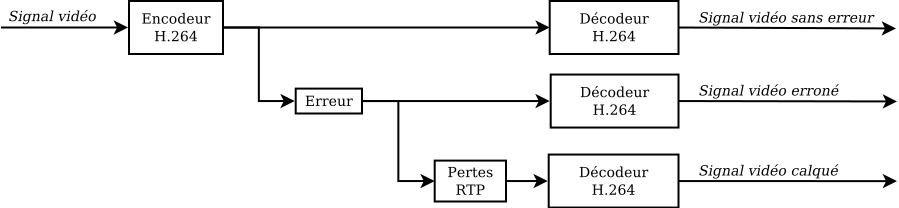
\includegraphics[width=0.97\linewidth]{images/EncoderDecoder.pdf} }
\caption[Diagramme des étapes du banc d'essai]{Diagramme des étapes du banc
d'essai.}
\label{fig-EncoderDecoder}
\end{figure}

Nous présentons, à la \fig{fig-EncoderDecoder}\footnote{Le diagramme de la
\fig{fig-EncoderDecoder} n'illustre qu'une partie du banc d'essai. Le diagramme
complet se trouve à l'annexe \ref{Ann-Setup} \page{Ann-Setup}.}, les étapes de
notre banc d'essai. Nous y observons qu'un signal vidéo est encodé, transmis,
puis décodé trois fois. La première opération de décodage décode les données
sans que celles-ci soient exposées à l’erreur. Cette étape est cruciale afin de
déterminer la dégradation visuelle engendrée par l’encodage du signal. Dans la
seconde opération, la séquence encodée est sujette à un motif d’erreur binaire
\ang{Bit Error Pattern} gaussien. Les données corrompues sont envoyées au
décodeur. S’il réussit à les décoder, celles-ci sont conservées, sinon la
sous-séquence est rejetée. Dans la dernière opération de décodage, la
sous-séquence corrompue est analysée par un module de détection de pertes RTP
\ang{RTP loss}. Celui-ci identifie et retire les paquets RTP corrompus. Les
données résultant de l’analyse de pertes RTP sont décodées. Lorsque le décodeur
s'aperçoit d'un paquet manquant, il utilise une approche de dissimulation
d’erreurs. Par exemple, il remplace la tranche manquante par son équivalent dans
la trame précédente\footnoteETS{Dans cet ouvrage, \textit{slice copy} a été
utilisé au détriment de \textit{motion copy}, car aucune implémentation
fonctionnelle de \textit{motion copy} n'était disponible. Lors de l'utilisation
de \textit{motion copy}, nous avons éprouvé des problèmes avec les versions~15.1
à 16.2 du décodeur inclus dans le \ltCodec. Ces problèmes sont connus et
confirmés par plusieurs forums Internet et catalogués dans le logiciel de suivi
de problèmes Mantis relié au \ltCodec~\citep{BUG}. C'est pour cette raison,
quoique notre ouvrage soit aussi compatible avec \textit{motion copy}, que nous
avons testé nos solutions avec \textit{slice copy}.} (\textit{slice copy},
traduit dans cet ouvrage par la locution tranche calquée).

Les séquences sont encodées et décodées à l'aide de la version~16.2 du
\ltCodec~\citep{JM}. Ce dernier, n'étant pas un produit commercial, a pour
objectif principal la démonstration de nouvelles fonctionnalités visant la norme
H.264. Notre banc d'essai est constitué de sous-ensembles de quatre trames
consécutives commençant à un emplacement aléatoire dans diverses séquences
vidéos. Ces sous-ensembles débutent par une trame \textit{intra} suivi de trois
trames \textit{inter} (IPPP). Nous retenons cinq sous-ensembles pour chaque
séquence de résolution QCIF contenue dans l'ensemble de séquences de référence
de l'Université l'État de l'Arizona~\citep{YUV}.

Dans le contexte d'applications mobiles, le débit est souvent fixe (typiquement
entre 64~kb/s et 128~kb/s pour les séquences QCIF). Cependant, pour simplifier
nos expérimentations, nous imposons plutôt un paramètre de quantification (QP)
fixe. Ceci élimine les variations de la qualité visuelle dues aux changements de
QP requis pour garder le débit fixe. Parmi les valeurs de 0 à 51 du paramètre de
quantification, nous avons retenu~: 16, 20, 24 et 28. Ces valeurs sont choisies,
car elles représentent un intervalle de données plausibles pour une application
mobile selon la bande passante disponible. De plus, nous n'avons pas retenu des
QP trop élevés (c.-à-d.~QP$~>30$), car la quantité de bits requis pour encoder
une trame QCIF est si minime qu’il arrive souvent que lesq taux d’erreurs
utilisés ne parviennent pas à briser un seul bit de la trame.

Les taux d'erreur binaire (BER) utilisés sont~: 0.0004, 0.0008, 0.0016, et
0.0032. Cet intervalle de taux est considérablement large et agressif par
rapport aux intervalles d'erreurs retrouvés dans la littérature de la norme
H.264~\citep{Stockhammer2003}. Nous avons choisi un tel intervalle pour obtenir
des résultats témoignant des gains possibles dans un grand nombre de conditions
d'erreur de transport. Le taux d'erreur utilisé est appliqué au niveau des bits
et non pas au niveau des paquets~\citep{Wenger2003} ou des blocs (comme dans les
ouvrages de dissimulation d'erreurs).

Seule la troisième trame (une trame P) est exposée à l'erreur. En ce qui
concerne l'ordonnancement de macroblocs flexible (FMO), deux types sont
employés~: dispersé \ang{dispersed} et entrelacé \ang{interlaced}. Tous deux
sont composés de deux tranches. À la \fig{fig-392} et \ref{fig-1752}, nous
présentons deux exemples d'erreurs pour chacun des types d'ordonnancement. Les
sous-séquences sont encodées à 30 images par seconde, tandis que les autres
paramètres sont propres au profil de base \ang{baseline} défini dans la norme
H.264. Le format de sortie est RTP et la résolution est QCIF, c'est-à-dire
$176\times 144$ pixels. Rappelons l'hypothèse, précédemment posée, que les
en-têtes NAL et RTP n'ont pas été exposés à l'erreur.

\begin{figure}[htb]
\fbox{\begin{varwidth}{\textwidth}\centering
\subfigure[Trame erronée]{
\includegraphics[width=0.46\linewidth]{images/badCarphoneInterleaved.png}
\label{fig-392-bad}
}
\subfigure[Erreur (amplifiée)]{
\includegraphics[width=0.46\linewidth]{images/diffCarphoneInterleaved.png}
\label{fig-392-err}
}
\end{varwidth}}
\caption[Erreur présente dans la sous-séquence \#392 du jeu de tests]{Exemple de
l'erreur présente dans la sous-séquence \#392 du jeu de tests. (Séquence~:
Carphone, QP=16 BER=0.0032, FMO=Entrelacé)}
\label{fig-392}
\end{figure}

\begin{figure}[htb]
\fbox{\begin{varwidth}{\textwidth}\centering
\subfigure[Trame erronée]{
\includegraphics[width=0.46\linewidth]{images/badCarphoneDispersed.png}
\label{fig-1752-bad}
}
\subfigure[Erreur (amplifiée)]{
\includegraphics[width=0.46\linewidth]{images/diffCarphoneDispersed.png}
\label{fig-1752-err}
}
\end{varwidth}}
\caption[Erreur présente dans la sous-séquence \#1752 du jeu de tests]{Exemple
de l'erreur présente dans la sous-séquence \#1752 du jeu de tests. (Séquence~:
Carphone, QP=16 BER=0.0032, FMO=Dispersé)}
\label{fig-1752}
\end{figure}

Notre banc d'essai est constitué d'un jeu de tests de 2720 sous-ensembles de
trames. Plus précisément, nous avons 1360 trames dispersées et 1360 trames
entrelacées. Ces 1360 trames proviennent de 17 séquences vidéos distinctes. Pour
chacune d'elles, cinq sous-séquences distinctes ont été utilisées. Celles-ci ont
été encodées avec nos quatre paramètres de quantification et exposées à nos
quatre taux d'erreur ($17 \times 5 \times 4 \times 4 = 1360$).

En ce qui concerne les données d'entrainement utilisées pour établir les
seuils, celles-ci proviennent du même banc d'essai, mais avec des trames de
départs aléatoires, distinctes de celles utilisées pour mesurer les performances
de nos solutions.

À la prochaine section, le banc d'essai sera employé pour déterminer la
résilience du décodeur inclus dans le \ltCodec. La
\sect{sec-ApprocheSelective} résume notre utilisation du banc d'essai pour
valider les approches sélectives de détection et de dissimulation d'erreur
proposées.

\FloatBarrier
\end{section}

\begin{section}{Analyse de la résilience aux erreurs du décodeur de référence H.264}
\label{sec-ResilienceDecodeur}
Dans certaines conditions, le décodeur inclus dans le \ltCodec~réussit à décoder
des séquences binaires corrompues. Cette découverte, initiatrice de notre effort
de recherche, a été réalisée très tôt dans nos expérimentations. Notons que, un
décodage réussi est pour nous l'opération de décoder une tranche corrompue qui
ne \textit{plante} pas le décodeur, sans pour autant garantir l'intégrité du
contenu en résulte. En d'autres mots, l'image issue du décodage d'une tranche
corrompue va souvent contenir de la dégradation visuelle (voir figures
\ref{fig-726-bad} \page{fig-726-bad}, \ref{fig-392-bad} \page{fig-392-bad} et
\ref{fig-1752-bad} \page{fig-1752-bad}). Le taux de décodages réussis varie, non
seulement selon le taux d'erreur binaire appliqué à la séquence, mais aussi
selon le paramètre de quantification (QP) utilisé lors de l'encodage. Ceci
s'explique par le fait qu'un QP plus faible force l'encodeur à utiliser plus de
bits pour encoder une trame; et plus il y a de bits sujets à erreur, plus la
probabilité de corruption de la trame augmente.

\begin{figure}
\fbox{\begin{varwidth}{\textwidth}\centering
\subfigure[Ordonnacement dispersé]{
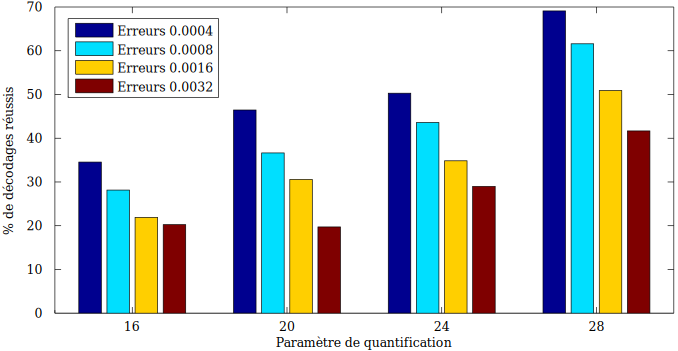
\includegraphics[width=0.97\linewidth]{images/decodingDispersed.pdf}
}\\
\subfigure[Ordonnacement entrelacé]{
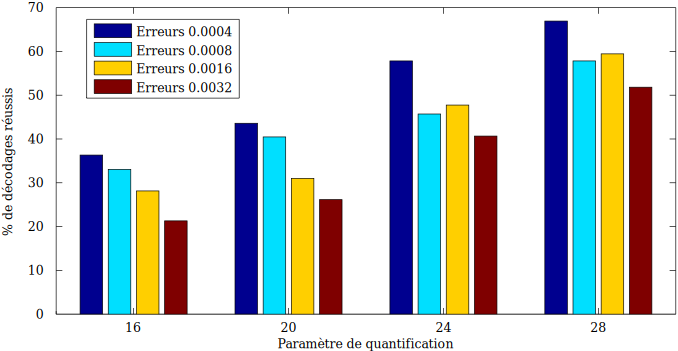
\includegraphics[width=0.97\linewidth]{images/decodingInterleaved.pdf}
}
\end{varwidth}}
\caption[Histogrammes des pourcentages de décodages réussis]{Histogrammes des
pourcentages de décodages réussis en fonction du paramètre de quantification
utilisé lors de l'encodage ainsi que du taux d'erreurs sur les bits (BER).}
\label{fig-Decodings}
\vspace{2em}
\end{figure}

Les histogrammes de la \fig{fig-Decodings} présentent les taux de décodages
réussis observés en fonction des paramètres de quantification et du taux
d'erreur sur les bits présents dans notre jeu de tests. Ces taux sont
intéressants, car ils confirment que le décodage des données corrompues peut
avoir un taux de réussite allant de 20~\% à 70~\%, selon les conditions. On peut
concevoir une stratégie de résilience à l'erreur, où une prochaine génération de
décodeurs seraient en mesure d'effectuer une tentative de décodage d'une tranche
corrompue, dans un environnement contrôlé (possiblement à l'aide d'un second
décodeur), afin d'éviter que le décodeur principal \textit{plante}.

\begin{figure}[htb]
\fbox{\begin{varwidth}{\textwidth}\centering
\subfigure[Trame Corrompue]{
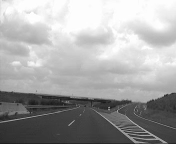
\includegraphics[width=0.30\linewidth]{images/ErrorFrame.png}
\label{fig-ErrorFrame}
}
\subfigure[Différentiel entre (a) et la trame non-erronée]{
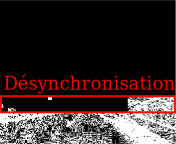
\includegraphics[width=0.30\linewidth]{images/Desync.pdf}
\label{fig-Desync}
}
\subfigure[Différentiel entre (a) et la trame précédente]{
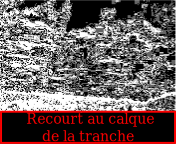
\includegraphics[width=0.30\linewidth]{images/Revert.pdf}
\label{fig-Revert}
}
\end{varwidth}}
\caption[Exemple du comportement du décodeur]{Exemple du comportement du
décodeur. En \subref{fig-Desync}, le différentiel de \subref{fig-ErrorFrame},
par rapport à la trame codée/décodée sans erreur, est utilisé pour démontrer la
désynchronisation. Le différentiel entre \subref{fig-ErrorFrame} et la trame
précédente permet de démontrer, en \subref{fig-Revert}, l'utilisation du calque
de tranche.}
\label{fig-DecoderBehavior}
\end{figure}

Lors du décodage d'une tranche corrompue, le décodeur inclus dans le
\ltCodec~fait la transition entre trois états distincts. Le résultat de ceux-ci
est illustré à la \fig{fig-DecoderBehavior}. Le premier état est celui du
décodage des bits de la tranche corrompue situés avant l'erreur. Cet état est
équivalent au décodage normal d'une trame. Il est illustré par la partie
supérieure, tout en noir (signifiant l'absence de différence), du
différentiel~\subref{fig-Desync} de la \fig{fig-DecoderBehavior}.

Par la suite, le décodeur décode le premier bit corrompu. Ceci cause une
désynchronisation des codes binaires de l'encodage entropique. Même si les
autres bits de la séquence sont valides, la désynchronisation fait en sorte
qu'ils sont associés à la mauvaise valeur dans la table de référence CAVLC. Le
décodeur interprète ces mauvaises valeurs, ce qui entraine une dégradation
visuelle dans l'image. Cette dégradation peut se manifester fortement, comme
c'est le cas dans l'image de la \fig{fig-726-bad}, ou être presque
imperceptible, comme c'est le cas dans la \fig{fig-ErrorFrame}. Afin de mieux
voir la dégradation visuelle de la \fig{fig-ErrorFrame}, elle est encadrée à la
\fig{fig-Desync}. C'est dans ce second état que le décodeur est le plus
vulnérable aux défaillances.

Le second état se termine lorsque le décodeur cesse d'insérer de la dégradation
visuelle dans l'image et utilise le contenu provenant de la tranche précédente.
Ce changement est illustré en~\ref{fig-Revert}. Ici, on suppose que le décodeur
est complètement désynchronisé; il ne sait que faire de ce qu'il décode; il
applique donc le contenu des blocs précédents, ce qui, grâce à la corrélation
temporelle, est le contenu de remplacement correct s'il y a absence de
mouvement. De plus, notons que dans l'image~\ref{fig-ErrorFrame}, il y a très
peu d'effets de blocs causés par la désynchronisation. Ceci est dû au filtre
antiblocs. Lorsqu'il est appliqué sur la trame, il identifie et lisse les
effets de blocs. Ceci explique aussi pourquoi, aux figures \ref{fig-392-bad} et
\ref{fig-392-err}, l'erreur se répand à la tranche non erronée. Dans ce cas, le
filtre antiblocs lisse le bloc erroné, ce qui répand l'erreur dans les blocs
avoisinants.

\FloatBarrier
\end{section}

\begin{section}{Analyse de l'approche sélective}
\label{sec-ApprocheSelective}
Comme démontré à la section précédente, l'image résultant d'une tranche
corrompue peut souvent être décodée. Cependant, celle-ci possède, à cause de la
désynchronisation du décodeur lors du décodage, une dégradation visuelle plus ou
moins importante. Elle peut toutefois être utilisée pour guider un algorithme de
dissimulation d'erreurs grâce à un nouveau type d'algorithme, proposé dans ce
mémoire, permettant la détection de la dégradation visuelle.

L'algorithme de détection présenté dans cet ouvrage est basé sur la mesure des
effets de blocs compensés par le mouvement (MCB), et détecte la dégradation
visuelle causant des effets de blocs absents de la trame précédente. La prémisse
de notre approche sélective est de déterminer entre le tranche calquée
(\fig{fig-726-sc} \page{fig-726-sc}) et la tranche corrompue (\fig{fig-726-bad}
\page{fig-726-bad}), celle qui produirait la meilleure dissimulation (c.-à-d.
qui produirait le meilleur PSNR par rapport à la trame de référence). Cette
opération peut être accomplie à deux niveaux~: celui de la tranche, à l'aide du
SDMCB, ou celui des blocs, avec le MCB. Nous présenterons tout d'abord la
configuration de notre banc d'essai conçu pour mesurer l'approche sélective. Par
la suite, la sous-\sect{sec-AnalyseSDMCB} présente les résultats obtenus avec le
SDMCB et la sous-\sect{sec-AnalyseMCB}, les résultats du MCB.
\LT{MCB, SDMCB et le PSNR sont présentés dans des séctions précédentes.}

\begin{figure}[htb]
\fbox{\centering
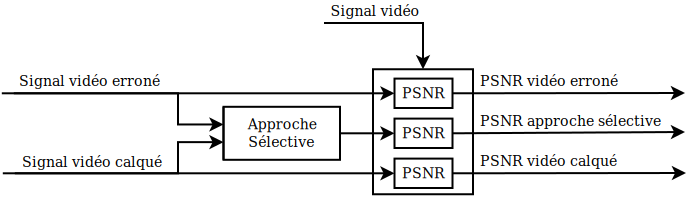
\includegraphics[width=0.97\linewidth]{images/SelectiveSetup.pdf}
}
\caption[Banc d'essai pour mesurer l'approche sélective]{Configuration du banc
d'essai pour mesurer l'approche sélective.}
\label{fig-SelectiveSetup}
\end{figure}

Tout d'abord, à l'aide du PSNR comme discriminant, nous mesurons, par rapport au
signal vidéo original, la qualité visuelle des dissimulations pour la tranche
calquée et la tranche corrompue. La \fig{fig-SelectiveSetup}\footnote{Le
diagramme de la \fig{fig-SelectiveSetup} n'illustre qu'une partie du banc
d'essai. Le diagramme complet se trouve à l'annexe \ref{Ann-Setup}
\page{Ann-Setup}.} démontre la configuration élaborée pour obtenir ces mesures.
Cette configuration s'ajoute à la suite de celle présentée à la
\fig{fig-EncoderDecoder} \page{fig-EncoderDecoder}. On y constate que le PSNR
est mesuré par rapport au signal vidéo de référence et qu'il est mesuré pour
l'image résultant du décodage de la tranche corrompue, pour le candidat de
dissimulation basée sur la tranche calquée et pour le résultat des approches
sélectives basées sur le SDMCB et MCB.

Par la suite, les résultats mesurés sur nos données d'essai sont présentés à la
\fig{fig-ScVsErroneous}. On y remarque une importante quantité de trames et de
blocs erronés qui possèdent un PSNR supérieur aux trames calquée. Cela
s'explique par le fait que, dans ces cas, la dégradation visuelle engendrée par
la désynchronisation du décodeur est moins importante que la variation
temporelle par rapport à la trame précédente, ce qui pénalise la tranche
calquée. En lien avec les trois états d'un décodeur traitant une tranche
corrompue, nous pouvons conclure que, dans l'état~1, la tranche endommagée va
produire un meilleur résultat que le calquage de la tranche. Dans l'état~2, la
tranche endommagée va produire un résultat inférieur à la tranche calquée.
Finalement, à l'état~3, les deux sont équivalents. La proportion de blocs
compris dans les états~1 et 2, l'intensité de la dégradation produite par le
décodeur ainsi que la variation temporelle par rapport à la trame précédente
sont les facteurs qui déterminent laquelle des deux trames constituera la
meilleure alternative.

\begin{figure}
\fbox{\begin{varwidth}{\textwidth}\centering
\subfigure[Distribution des trames corrompues (cercles rouges) par rapport aux
trames calquées (ligne bleue)]{
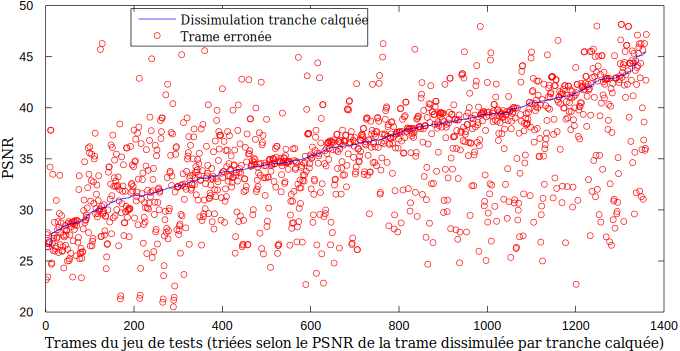
\includegraphics[width=0.97\linewidth]{images/scVsErroneous.pdf}
\label{fig-scVsErroneous}
}\\
\subfigure[Distribution des blocs issus des trames corrompues (cercles magenta)
par rapport aux blocs issus des trames calquées (ligne noire). À des fins de
visualisation, seulement un bloc sur dix est affiché.]{
\includegraphics[width=0.97\linewidth]{images/ScVsErroneousBlocks.pdf}
\label{fig-scVsErroneousBlocks}
}
\end{varwidth}}
\caption[PSNR de la trame erronée et de la dissimulation par tranche
calquée]{Visualisation de la distribution des valeurs du PSNR de la trame erronée et de la dissimulation par tranche calquée.}
\label{fig-ScVsErroneous}
\vspace{2em}
\end{figure}

Plus précisément, les mesures obtenues de notre banc d'essai nous permettent de
conclure que l'image résultant du décodage de la tranche corrompue offre un
PSNR plus élevé dans 44~\% des cas pour l'ordonnancement dispersé et 49~\% pour
l'entrelacé. Pour ces trames, on observe respectivement des gains moyens de
2.12~dB et 1.68~dB par rapport à leurs trames équivalentes calquées. De manière
similaire, les blocs issus de trames corrompues sont supérieurs dans 42~\% des
cas pour l'ordonnancement dispersé et 49~\% pour l'entrelacé. Ces blocs
produisent, pour les approches d'ordonnancement précédentes, des gains moyens de
1.44~dB et 1.02~dB.

\LT{Annexer les graphes pour chaque BER et QP.}

Bref, nous avons déjà démontré qu'il est possible de réussir à décoder des
tranches erronées. Ce que nous venons de démontrer, dans cette section, est
qu'une quantité importante des images résultant d'un tel décodage exhibent une
fidélité visuelle supérieure au calque de cette tranche (approche couramment
employée par le décodeur fourni avec le \ltCodec).

\FloatBarrier
\begin{subsection}{Approche sélective SDMCB} \label{sec-AnalyseSDMCB}
Maintenant, toujours avec la même configuration du banc d'essai, mesurons
l'aptitude du SDMCB à identifier le meilleur candidat entre la trame corrompue
et la dissimulation par tranche calquée. Pour ce faire, nous utilisons une
taille de bloc $B=16$ (vu notre indépendance au train de bits, nous ne
connaissons pas la taille exacte des blocs) et un seuil d'effet de bloc $T_b =
5000$. La taille des macroblocs étant $16\times 16$, ceci nous permet de
conclure que s'il y a erreur, les effets de blocs vont souvent se manifester en
bordure de macroblocs. La valeur du seuil $T_b$ est obtenue avec des données
d'essai provenant du même jeu de test, mais avec des trames de départ
différentes.

Deux exemples de trames et de leur pointage MCB sont présentés aux
figures~\ref{fig-SilentInter} et \ref{fig-SilentDisp}. Dans les deux cas, on
constate que l'erreur de la trame endommagée (\ref{fig-SilentBadPerfDiff} et
\ref{fig-SilentDispBadPerfDiff}) est moins nuisible que celle de la trame
calquée (\ref{fig-SilentFcPerfDiff} et \ref{fig-SilentDispFcPerfDiff}). Ceci se
refléte dans le pointage SDMCB. Ce dernier permet d'identifier la trame avec le
moins d'erreurs, dans un contexte où la trame de référence n'est pas disponible.

\begin{figure}[htb]
\fbox{\begin{varwidth}{\textwidth}\centering
\subfigure[Trame endommagée ($SDMCB = 9983$)]{
\includegraphics[width=0.47\linewidth]{images/silentBad.png}
\label{fig-SilentBad}
}
\subfigure[Trame calquée ($SDMCB = 13142$)]{
\includegraphics[width=0.47\linewidth]{images/silentFc.png}
\label{fig-SilentFc}
}
\subfigure[Différentiel trame erronée et trame de référence]{
\includegraphics[width=0.47\linewidth]{images/silentBadPerfDiff.png}
\label{fig-SilentBadPerfDiff}
}
\subfigure[Différentiel trame calquée et trame de référence]{
\includegraphics[width=0.47\linewidth]{images/silentFcPerfDiff.png}
\label{fig-SilentFcPerfDiff}
}
\end{varwidth}} 
\caption[Pointages SDMCB obtenus par rapport à l'erreur (dispersé)]
{Visualisation des pointages SDMCB obtenus par rapport à l'erreur présente dans
les trames. (Séquence : Silent, QP=20 BER=0.0008, FMO=Dispersé)}
\label{fig-SilentInter}
\end{figure}

\begin{figure}[htb]
\fbox{\begin{varwidth}{\textwidth}\centering
\subfigure[Trame endommagée ($SDMCB = 9373$)]{
\includegraphics[width=0.47\linewidth]{images/silentDispBad.png}
\label{fig-SilentDipsBad}
}
\subfigure[Trame calquée ($SDMCB = 15564$)]{
\includegraphics[width=0.47\linewidth]{images/silentDispFc.png}
\label{fig-SilentDispFc}
}\\
\subfigure[Différentiel trame erronée et trame de référence]{
\includegraphics[width=0.47\linewidth]{images/silentDispBadPerfDiff.png}
\label{fig-SilentDispBadPerfDiff}
}
\subfigure[Différentiel trame calquée et trame de référence]{
\includegraphics[width=0.47\linewidth]{images/silentDispFcPerfDiff.png}
\label{fig-SilentDispFcPerfDiff}
}
\end{varwidth}} 
\caption[Pointages SDMCB obtenus par rapport à l'erreur (entrelacé)]
{Visualisation des pointages SDMCB obtenus par rapport à l'erreur présente dans
les trames. (Séquence : Silent, QP=16 BER=0.0004, FMO=Entrelacé)}
\label{fig-SilentDisp}
\end{figure}

\begin{figure}[htb]
\fbox{\begin{varwidth}{\textwidth}\centering
\subfigure[Ordonnancement dispersé]{
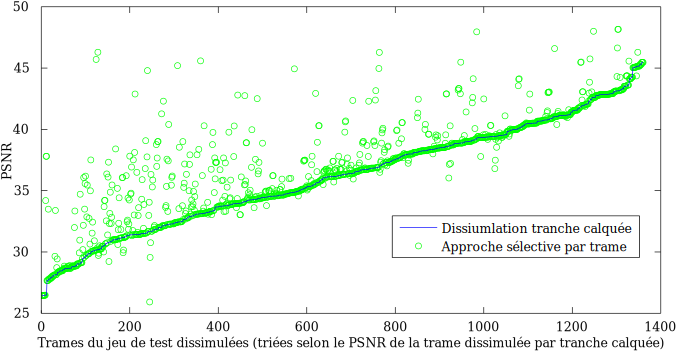
\includegraphics[width=0.97\linewidth]{images/selectiveSliceCopyDispersed.pdf}
\label{fig-sliceCopyDispersed}
}\\
\subfigure[Ordonnancement entrelacé]{
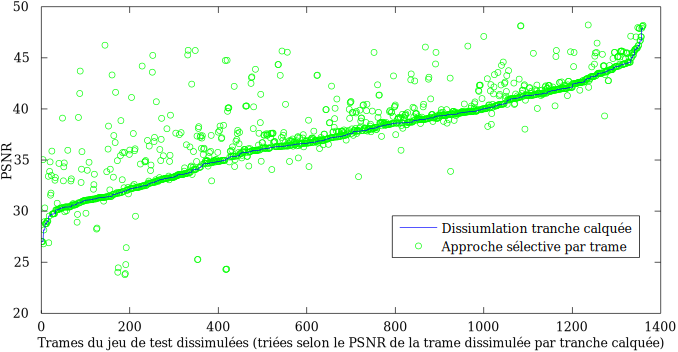
\includegraphics[width=0.97\linewidth]{images/selectiveSliceCopyInterleaved.pdf}
\label{fig-sliceCopyInterleaved}
}
\end{varwidth}} 
\caption[PSNR de l'approche sélective basée sur SDMCB]{Visualisation de la
distribution du PSNR de l'approche sélective basée sur SDMCB (cercles verts) à l'égard de la dissimulation par tranche calquée (ligne
bleue).}
\label{fig-SelectiveSliceCopy}
\end{figure}

Les résultats obtenus sont présentés à la \fig{fig-SelectiveSliceCopy}. La
\fig{fig-sliceCopyDispersed} montre que l'approche sélective, dans le cadre d'un
ordonnancement dispersé, fait le bon choix dans 81~\% des cas. Pour ceux-ci, un
gain moyen de 1.98~dB est mesuré, tandis que pour l'ensemble de la séquence le
gain moyen est de 0.72~dB. Les choix de l'approche sélective offrent un PSNR
supérieur aux trames dissimulées par calquage de tranche dans 31~\% des cas.
Pour la \fig{fig-sliceCopyInterleaved}, la bonne trame est choisie dans 86~\%
des cas. Il en résulte un gain moyen de 1.24~dB pour celles-ci. Sur l'ensemble
des trames, le gain moyen est de 0.65~dB et un PSNR supérieur au calquage de
trame est obtenu dans 43~\% des cas.

\FloatBarrier
\end{subsection}
\begin{subsection}{Approche sélective MCB}
\label{sec-AnalyseMCB}
Le niveau de granularité plus fin de l’approche sélective MCB est son attrait
principal. En remplaçant uniquement les blocs endommagés, on maximise l’usage
des données correctement décodées.

Sans altérer la configuration de notre banc de test, nous mesurons l'aptitude du
MCB à identifier le meilleur bloc candidat entre ceux provenant de la trame
corrompue et ceux, de la dissimulation par tranche calquée. Pour ce faire, nous
réutilisons la taille de bloc $B=16$ et le seuil d'effet de bloc $T_b = 5000$.

Aux figures~\ref{fig-AkiyoBlockSel} et~\ref{fig-SilentBlockSel}, on constate
les gains en PSNR issus de l'approche sélective. Ces gains proviennent des
choix de blocs provenant de la trame calquée(\ref{fig-AkiyoFcChoice},
\ref{fig-ChoiceFcInter}) et de la trame endommagée(\ref{fig-AkiyoBadChoice},
\ref{fig-ChoiceBadInter}). Dans les deux cas, l'approche sélective écarte les
blocs possédant une détérioration visuelle en faveur du bloc analogue dans
l'autre trame.

\begin{figure}[htb]
\fbox{\begin{varwidth}{\textwidth}\centering
\subfigure[Trame endommagée (PSNR = 25.35~dB)]{
\includegraphics[width=0.45\linewidth]{images/akiyoBadDisp.png}
\label{fig-AkiyoBad}
}
\subfigure[Trame calquée (PSNR = 39.84~dB)]{
\includegraphics[width=0.45\linewidth]{images/akiyoFcDisp.png}
\label{fig-AkiyoFc}
}
\subfigure[Blocs choisies dans la trame endommagée]{
\includegraphics[width=0.45\linewidth]{images/choiceBadDisp.png}
\label{fig-AkiyoBadChoice}
}
\subfigure[Blocs choisies dans la trame calquée]{
\includegraphics[width=0.45\linewidth]{images/choiceFcDisp.png}
\label{fig-AkiyoFcChoice}
}
\subfigure[Trame sélective par blocs (PSNR = 44.07~dB)]{
\includegraphics[width=0.45\linewidth]{images/akiyoSelDisp.png}
\label{fig-AkiyoSel}
}
\end{varwidth}} 
\caption[Blocs choisis dans la trame corrompue et la trame calquée par
l'approche MCB (dispersé)]{Visualisation des blocs choisies dans la trame
corrompue et la trame calquée par l'approche MCB. (Séquence : Akiyo, QP=16 BER=0.0008,
FMO=Dispersé)}
\label{fig-AkiyoBlockSel}
\end{figure}

\begin{figure}[htb]
\fbox{\begin{varwidth}{\textwidth}\centering
\subfigure[Trame endommagée (PSNR = 24.76~dB)]{
\includegraphics[width=0.45\linewidth]{images/silentBadInter.png}
\label{fig-SilentBadInter}
}
\subfigure[Trame calquée (PSNR = 36.38~dB)]{
\includegraphics[width=0.45\linewidth]{images/silentFcInter.png}
\label{fig-SilentFcInter}
}
\subfigure[Blocs choisies dans la trame endommagée]{
\includegraphics[width=0.45\linewidth]{images/choiceBadInter.png}
\label{fig-ChoiceBadInter}
}
\subfigure[Blocs choisies dans la trame calquée]{
\includegraphics[width=0.45\linewidth]{images/choiceFcInter.png}
\label{fig-ChoiceFcInter}
}
\subfigure[Trame sélective par blocs (PSNR = 38.94~dB)]{
\includegraphics[width=0.45\linewidth]{images/silentSelInter.png}
\label{fig-SilentSelInter}
}
\end{varwidth}} 
\caption[Blocs choisies dans la trame corrompue et la trame calquée par
l'approche MCB (entrelacé)]{Visualisation des blocs choisies dans la trame
corrompue et la trame calquée par l'approche MCB. (Séquence : Silent, QP=16
BER=0.0008, FMO=Entrelacé)}
\label{fig-SilentBlockSel}
\end{figure}

\begin{figure}[htb]
\fbox{\begin{varwidth}{\textwidth}\centering
\subfigure[Ordonnancement dispersé]{
\includegraphics[width=0.97\linewidth]{images/SelectiveSliceCopyBlocksDispersed.pdf}
\label{fig-selectiveSliceCopyBlockDispersed}
}\\
\subfigure[Ordonnancement entrelacé]{
\includegraphics[width=0.97\linewidth]{images/SelectiveSliceCopyBlocksInterleaved.pdf}
\label{fig-selectiveSliceCopyBlockInterleaved}
}
\end{varwidth}}
\caption[PSNR issue des blocs résultants de l'approche sélective basée sur
MCB]{Visualisation de la distribution du PSNR issue des blocs résultants de
l'approche sélective basée sur MCB (cercles cyan) à l'égard de ceux produits par
la dissimulation par tranche calquée (ligne bleue).}
\label{fig-SelectiveSliceCopyBlocks}
\end{figure}

Les résultats obtenus sont présentés à la \fig{fig-SelectiveSliceCopyBlocks}. La
\fig{fig-selectiveSliceCopyBlockDispersed} démontre que l'approche sélective MCB
choisit le bon bloc dans 88~\% de cas, ce qui produit un gain moyen de 0.86~dB
sur l'ensemble des trames avec un ordonnancement de type dispersé. Pour
l'ordonnancement entrelacé (\fig{fig-selectiveSliceCopyBlockInterleaved}),
l'approche sélective MCB effectue le bon choix dans 91~\% des cas, permettant un
gain moyen de 0.69~dB.

\FloatBarrier
\end{subsection}

À l'aide de la \fig{fig-FrameDistribution}, nous sommes en mesure d'analyser la
distribution des PSNR résultant de la trame erronée, de la dissimulation par
tranche calquée et des approches sélectives. Cette figure expose la variation du
nombre de trames selon des intervalles de 5~dB de PSNR. Ces intervalles
s'étalent de 20~dB à 50~dB, permettant ainsi de visualiser la variation de la
qualité visuelle issue de chaque approche.

Commençons l'analyse en soulignant la présence d'une importante quantité de
trames erronées dans les intervalles de faible qualité, où le PSNR est inférieur
à 30 (les intervalles centrés autour de 20 et 25). Pour ces intervalles, nous
constatons, autant dans l'histogramme de la \fig{fig-SelectiveHistDispersed} que
\ref{fig-SelectiveHistInterleaved}, que la majorité de ces trames sont
dissimulées par les tranches calquées et les approches sélectives.

Poursuivons l'analyse des approches sélectives avec le constat suivant~: pour
l'intervalle centré autour de 30~dB, le nombre de trames liées aux approches
sélectives est inférieur à celui des trames liées à la dissimulation par tranche
calquée. Cette observation n'est pas due à une perte de qualité, mais bien à une
augmentation de la qualité, car on retrouve ces trames dans les intervalles
supérieurs. Pour ces intervalles, les approches sélectives produisent un plus
grand nombre de trames que la dissimulation par tranche calquée.

Grâce à ces observations, nous sommes en mesure de conclure que les approches
sélectives produisent de meilleurs résultats en exploitant les trames erronées
de haute qualité visuelle, tout en évitant les trames erronées de mauvaise
qualité. En ce qui a trait à la comparaison des approches sélectives, l'approche
sélective MCB offre un plus grand nombre de trames de qualité visuelle pour les
intervalles de 35~dB et 40~dB vis-à-vis SDMCB. Cependant, l'approche sélective
SDMCB se reprend dans l'intervalle de 45~dB. Cette reprise est attribuée au fait
que le remplacement de blocs sporadiques dans une trame peut engendrer une perte
de qualité causée par le mauvais arrimage des valeurs de pixels en frontière de
bloc. Cette légère dégradation réduit le nombre de trames de très haute qualité.
Toutefois, à des niveaux de 40dB et plus, la différence de qualité est souvent
imperceptible. Pour éviter d'avoir à manipuler des valeurs de PSNR infinies,
nous avons saturé le PSNR à 75~dB. Cette valeur a été choisie, car elle
surpassait l'ensemble des valeurs mesurées, comme on peut le constater à la
\fig{fig-SelectiveSliceCopyBlocks}.

\begin{figure}[htb]
\fbox{\begin{varwidth}{\textwidth}\centering
\subfigure[Ordonnancement dispersé]{
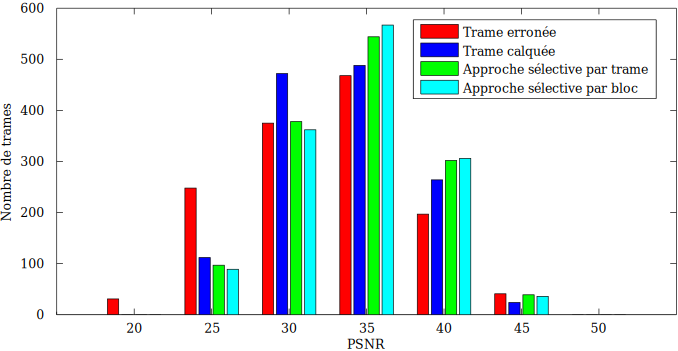
\includegraphics[width=0.97\linewidth]{images/SelectiveHistDispersed.pdf}
\label{fig-SelectiveHistDispersed}
}\\
\subfigure[Ordonnancement entrelacé]{
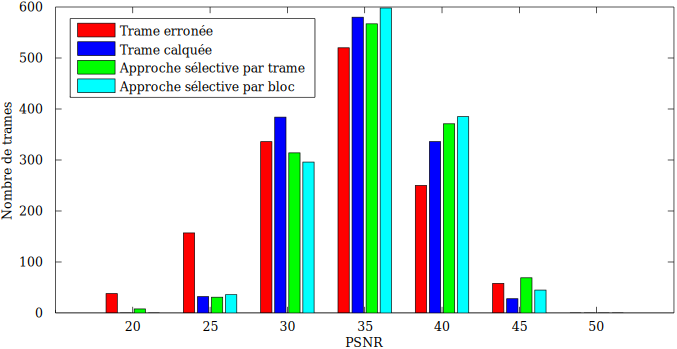
\includegraphics[width=0.97\linewidth]{images/SelectiveHistInterleaved.pdf}
\label{fig-SelectiveHistInterleaved}
}
\end{varwidth}}
\caption[Histogrammes des PSNR des trames]{Histogrammes des PSNR des trames,
avec des intervalles de 5~dB, centrés à chaque incrément de 5~dB, à partir de 20~dB. Les trames considérées sont
celles résultantes~: du décodage de la trame erronée (rouge), du calquage de
tranche (bleu), de l'approche sélective par tranche (vert) ainsi que
l'approche sélective par bloc (cyan).} 
\label{fig-FrameDistribution}
\end{figure}

\begin{table}[!htb]
\caption[Résumé du PSNR moyen obtenu par les diverses approches
présentées]{Résumé du PSNR moyen obtenu par les diverses approches présentées dans cette section sur le jeu de tests.}
\label{tab-ResumeSelectif}
\small
\centering
\begin{tabular}{| l | c | c |}
 \hline
 \multirow{2}{*}{\textbf{Approche}} & \textbf{PSNR Moyen}& \textbf{PSNR Moyen}\\
 &\textbf{dispersé (dB)}&\textbf{entrelacé (dB)}\\
 \hline
 Encodée (sans erreur) & 41.218222 & 41.200377\\
  \hline
 Sélective par bloc (avec référence) & 37.689039 & 38.528986\\
  \hline
 Sélective par tranche (avec référence) & 37.117712 & 38.082769\\
  \hline
 Sélective MCB & \textbf{37.034840} & \textbf{37.951004}\\
  \hline
 Sélective SDMCB & \textbf{36.901414} & \textbf{37.911514}\\
  \hline
 Dissimulation tranche calquée & 36.179630 & 37.263033\\
  \hline
 Trame corrompue & 35.068784 & 36.075526\\
 \hline   
\end{tabular}
\end{table}

Le tableau~\ref{tab-ResumeSelectif} résume les résultats présentés dans cette
section. De par ces résultats, nous sommes en mesure de conclure deux choses. La
première est que les trames issues du décodage de séquences corrompues possèdent
une qualité visuelle importante et exploitable. La seconde est que les approches
sélectives issues de nos travaux et appliquées à un tel décodage peuvent guider
la détection d'erreurs et servir à l'amélioration de la dissimulation. De plus,
le tableau valide que nos algorithmes de sélection sont en mesure d’alterner
efficacement entre la trame calquée et la trame corrompue afin d’offrir une
dissimulation supérieure à celle offerte par le calquage de trame. En derniers
lieux, les valeurs obtenues avec une sélection guidée par la trame de référence
sont présentées dans le tableau~\ref{tab-ResumeSelectif}. Ceci a pour but
de relativiser les résultats de nos approches sélectives sans référence.
\end{section}

\end{chapter}